\documentclass{article}
\usepackage{amsmath}
\usepackage{amssymb}
\usepackage{amsthm}
\usepackage{xcolor}
\usepackage{graphicx}
\newcommand\todo[1]{\textcolor{red}{#1}}

\newtheorem*{thm}{Theorem}
\newtheorem*{defn}{Definition}
\newtheorem*{pf}{Proof}

\title{First Steps into Topology}
\author{Cristóbal Sciutto}

\begin{document}
\maketitle

\section{Introduction}
This is intended to be a short venture into topology in, starting from
elementary real analysis, e.g. Stanford's Math 115.  My initial goal was to
reach some important results of differential topology, such as Brouwer's
fixed-point theorem and the hairy-ball theorem. However, making sure one is
rigorous leads to considerably slower progress than expected. Consequently, this
paper only takes the first couple of steps in that direction. The most important
lesson was realizing how a change in abstraction can lead to more
intuitive definitions of concepts, as per the fourth section of this paper,
in which I redefine convergence and continuity without $\epsilon-\delta$.

\section{A refresher on metric spaces}
In class, we were introduced to some basic concepts of metric spaces. These are
a special case of a topological space, and will provide a good starting point.
Let's remember the definitions, and see where we can generalize.

\begin{defn}[Metric Space]
A metric on a set $S$ is a function $d:S \rightarrow S$ satisfying:
\begin{enumerate}
\item (Identity of Indiscenibles) $d(x, y) = 0 \iff x = y$
\item (Symmetry) $d(x, y) = d(y, x)$
\item (Triangle Inequality) $d(x, y) + d(y, x) \geq d(x, z)$
\end{enumerate}
A metric space is set $S$ with a metric $d$: $(S, d)$.
\end{defn}

The metric space we are most acquantied with is defined over $\mathbb{R}^2$ with the
metric $d(x,y) = \sqrt{(x_1 - y_1)^2 + (x_2 - y_2)^2}$, i.e. Euclidean space.
This is easily extended to $\mathbb{R}^n$ by defining $d(x, y) = \sqrt{\sum_i(x_i -
y_i)^2}$. These Euclidean spaces will serve as our main examples in this
exposition of topology, as they come the most naturally to the student who
is just now dipping their toes into pure mathematics.

From there, we formalized a series of definitions related to openness of sets.
We started with the notion of a neighborhood around a point.

\begin{defn}[Neighborhood]
The neighborhood of point $p \in S$ is a ball with center $p$ and radius $r > 0$:
$B_d(p; r) = \{x \in S \mid d(x, p) < r\}$.
\end{defn}

For our familiar case of Euclidean space, this is the definition of a circle or
sphere centered around the point. We say $x$ is in the \textit{neighborhood} of
$p$ if $x \in B_d(p; r)$ for some $r$. Using this definition, we can define the
rest of the needed concepts. For the following definitions, let $E$ be a subset
of $S$.

\begin{defn}[Interior] 
$y\in E$ is interior if there exists a finite ball centered on $y$ contained in
    $E$, i.e. there exists an $r>0$ such that $x \in B_d(y; r) \implies x \in E$.
\end{defn}

\begin{defn}[Open] 
$E$ is open if all points in $E$ are interior.
\end{defn}

\begin{defn}[Closed] 
$E$ is closed if the complement of $E$ is open.
\end{defn}

An easy way to think of these definitions is to consider a closed-loop on
$\mathbb{R}^2$. All points inside the loop are interior. On the other hand, points on
the border of the loop are exterior. No matter how small the radius, there's
always a part of the ball outside of the region.

\begin{figure}[!htb]
  \center{
\includegraphics[width=0.2\textwidth] {figs/edge_is_not_interior.png}}
    \caption{\label{fig:edge} The edge is not interior. }
\end{figure}

The loop with its border is closed. The loop without its border is open.
Nevertheless, it's important to note that open and closed are not opposite. A
set can be both open and closed, open and not closed, closed and not open, or
neither open nor closed. For the first example, consider the empty set or all
of $\mathbb{R}^2$. For the last example, consider $[0, 1)$.

\section{What is a topology?}

From this definition of open sets, we can construct our definition of a
metric topological space.

\begin{defn}[Metric Topology]
The metric topology $\tau_d$ on $(S, d)$ is the set of all open sets in $S$.
\end{defn}

Now, you might be asking what a general topology is. In our case, we defined
open in terms of neighborhoods, which was in turn defined in terms of our
metric. While this was convenient for our real analysis class, the concept of
of openness actually comes before neighborhood. This will take a bit of work,
but we shall come full circle.

\begin{defn}[General Topology]
A topology $\tau$ of a set $S$ is subset of the powerset of $S$,
$\mathcal{P}(s)$, satisfying:
\begin{enumerate}
\item The empty set and $S$ are elements of $\tau$
\item All unions of elements of $\tau$ are in $\tau$
\item Finite intersections of elements of $\tau$ are in $\tau$
\end{enumerate}
We call the elements of $\tau$ open sets and the pair $(S, \tau)$ a topological
space.
\end{defn}

As an example, consider the set $S = \{1, 2, 3\}$. We note that $$\tau =
\{\emptyset, \{1\}, \{2\}, \{1, 2\}, \{1, 2, 3\}\}$$ is a topology satisfying the
properties above.

Note how this definition is independent of a metric. We've declared the open
sets as the sets of the topology. In this exposition, we shall focus on the
\textit{metric topologies}, so we should show that they satisfy the general
requirements stipulated above.

\begin{thm}
    Metric topologies are general topologies.
\end{thm}

\begin{pf}
Let $\tau$ be the open sets of $S$. We shall show that $\tau$ satisfies the
general topology properties delineated above.

\begin{enumerate}
\item The empty set is vacuously open. If $x \in S$, then $B_d(x; 1)$. Hence,
all points in $S$ are interior, and $S$ is open.
\item Let $x \in U = \bigcup_i U_i$. In particular, $x \in U_j$ for some $j$. Since
$U_j$ is itself open, then there exists $\epsilon$ such that $B_d(x; \epsilon)
\in U_j$. But $B_d(x; \epsilon) \in U$. Therefore, all points in $U$ are
interior and $U$ is open.
\item Let $x \in I = \bigcap_i I_i$. For each $I_i$, there exists $\epsilon_i$
such that $B_d(x; \epsilon_i) \in I_j$. If we let $\epsilon =
\min_i(\epsilon_i)$, then $B_d(x; \epsilon) \in I$. Hence, all points in $I$
are interior and $I$ is open.
\end{enumerate}
\end{pf}

Thus, one big takeaway is that topological spaces are a superset of metric
spaces. Topology uses the notion of an open set to talk about spaces that aren't
clearly measurable. For us, the notion of a neighborhood will remain strongly
linked to our $B_d(p;r)$ regions. However, a central move in topology is to
segregate this connection.

\begin{defn}[Neighborhood, redefined]
    The neighborhood of $x$ is an open set $U$ containing $x$.
\end{defn}

With this sleight-of-hand, we will be able to re-introduce several notions from
real analysis such as convergence and continuity, but applicable to a larger
domain of spaces, e.g. a torus.

\section{Convergence and continuity without $\epsilon$-$\delta$.}

In this section, I'll redefine the notions of convergence and continuity in the
language of topology. One small note: in topology, we usually refer to
functions as maps. There are some small differences, but for our purposes, one
can think of them as equivalent.

Let's recall our definition of convergence:
\begin{defn}[Analytical Convergence]
    Let $(s_n)$ be a sequence of terms in metric space $S$ with metric $d$. We
    say $(s_n)$ converges to $s$ if for any $\epsilon > 0$ there is an
    $N$ such that $$n>N \implies d(s_n, s) < \epsilon$$
\end{defn}

To rephrase it in topological terms, we want to express the notion of getting
arbitratily closed using just open sets. No matter how small the region you give
me around the limiting point, I can still find a large enough place to start in
my sequence such that all my terms are in that region.
\begin{defn}[Topological Convergence]
    We say $(s_n)$ converges to $s$ if for any neighborhood $U$ of $s$, there is an
    $N$ such that $$n>N \implies s_n \in U$$
\end{defn}

For the case of Euclidean space, taking neighborhood to be $B_d(s;\epsilon)$
makes the definitions equivalent. We can do a similar translation for the
notion of continuity.

\begin{defn}[Continuity at a point]
    $f: M \rightarrow N$ is continuous at $x_0$ if for all $\epsilon > 0$ there
    is a $\delta > 0$ such that $$\mid x-x_0 \mid < \delta \implies 
    \mid f(x)-f(x_0) \mid  < \epsilon$$
\end{defn}

We can extend the class definition to a general metric space, which will provide
a nicer segue to the topological defintion.

\begin{defn}[Analytical Continuity]
    Let $M$ and $N$ be metric spaces with associated metrics $d_M$ and $d_N$.
    Then $f: M \rightarrow N$ is continuous if for all $\epsilon > 0$ there is a
    $\delta > 0$ such that $$d_X(x, y) < \delta \implies d_Y(f(x), f(y)) <
    \epsilon$$
\end{defn}

\begin{defn}[Topological Continuity]
    Let $(M, \tau_M)$ and $(N, \tau_N)$ be topological spaces. Then a map $f: M
    \rightarrow N$ is continuous if for all $V \in \tau_N$, if $U$ is the
    pre-image of $V$, then $U \in \tau_M$.
\end{defn}

This can be more loosely stated as ``preimages of open sets are open
sets.'' Before proceeding blindly, let's make sure this at lines up with
our prior definition of continuity from class.

\begin{thm}
    For the Euclidean topological space $(\mathbb{R}, d, \tau)$, the topological
    definition of continuity implies the  $\epsilon$-$\delta$
    definition of continuity.
\end{thm}

\begin{figure}[!htb]
  \center{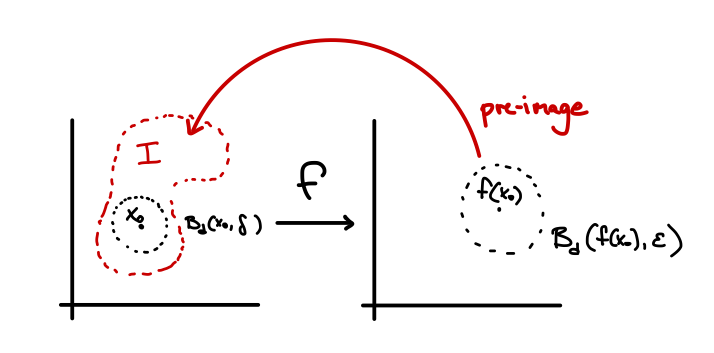
\includegraphics[width=\textwidth] {figs/continuity.png}}
    \caption{\label{fig:continuity} Visual proof of continuity. }
\end{figure}

\begin{pf}
    Consider $x_0 \in \mathbb{R}$ and its image $f(x_0) \in \mathbb{R}$ under
    continuous map $f$. Choose $\epsilon$. Note $B_d(f(x_0); \epsilon)$ is an
    open set $\in \mathbb{R}$. Since $f$ is topologically continuous, the
    preimage $I$ of $B_d(f(x_0); \epsilon)$ is also an open-set.  Hence, all
    points in $I$ are interior. In particular, $x \in I$ since $f(x_0) \in
    B_d(y;\epsilon)$.  Therefore, there exists a $\delta$ such that
    $B_d(x_0;\delta) \subseteq I$.

    Now consider an arbitrary point $p \in B_1(x_0;\delta) \subseteq I$. Since
    $I$ is the pre-image of $B_1(f(x_0); \epsilon)$, it follows that $f(p)
    \in B_1(f(x_0); \epsilon)$.
    Expanding out the definitions of 1-balls for when $d=1$, we have:
    for all $\epsilon$ there exists a $\delta$ such that $\mid x - x_0 \mid <
    \delta \implies \mid f(x) - f(x_0) \mid < \epsilon$.
\end{pf}

It is important to note that even if $f$ is continuous, there is no guarantee that
the inverse $f^{-1}$ is continuous. Consider the topologies $S = T
= \{1, 2\}$, $\tau_S = \{\emptyset, \{1\}, \{2\}, \{1, 2\}\}$, and $\tau_T =
\{\emptyset, \{1, 2\}\}$. If we define $f: S \rightarrow T$ as $f(1) = 2$
and $f(2) = 1$, then $f$ is continuous, however the inverse is not. Note that
the preimage of $\{1, 2\}$ under $f^{-1}$ is $\{1, 2\} \not\in
\tau_T$, hence the preimage of an open set is not an open set.

\section{Homeomorphisms and Manifolds}

In the study of cardinalities, we established bijections as functions that
preserve cardinality. This allowed us to reason about sets by referencing a
different set whose properties we already understood. For metric spaces, it
makes sense to study functions which preserve distances, called
\textit{isometries}. For the case of topologies, we studys homeomorphism as
they define a mapping (morphism) which maps similar (homeo) topological spaces
onto each other.

\begin{defn}[Homeomorphism]
    A map $f$ between topological spaces $(S, \tau_S)$ and $(T, \tau_T)$ is
    called a homeomorphism if $f$ is (1) one-to-one, (2) onto, (3) f is
    continuous, and (4) $f^{-1}$ is continuous.
\end{defn}

When you hear about topology in popular math books, the usual reference is to
toruses and coffee mugs being topologically equivalent, as one can smoothly
squish the mug into a torus (were they made out of Play-Doh). These kind of
transformations are precisely the one's defined by homeomorphisms.

Now we define the central object we will by studying: manifolds. These are a
kind of topological space, with the added constraint that they can be
``charted,'' like a map of the world. For example, a space is a
3-dimensional manifold, if we can draw it on a globe while preserving local
properties. To formalize this notion, we use our defintion of homeomorphism to
define manifolds as spaces that are locally Euclidean.

\begin{defn}[Manifold]
    A topological space $(S, \tau)$ is called a $d$-dimensional manifold if
    each for each point $p \in S$, there is an open set $U$ containing it,
    along with an associated homeomorphic map $f: U\rightarrow \mathbb{R}^d$.
\end{defn}

Some examples in the Euclidean-metric topological space:
\begin{enumerate}
    \item Torus: let $M$ be the points of a torus. Since $M \subset
        \mathbb{R}^3$, we can induce a topology onto the torus. Each open set in
        that manifold is homeomorpic to a Euclidean plane. Hence, it is a
        2-dimensional manifold.
\end{enumerate}

\begin{figure}[!htb]
  \center{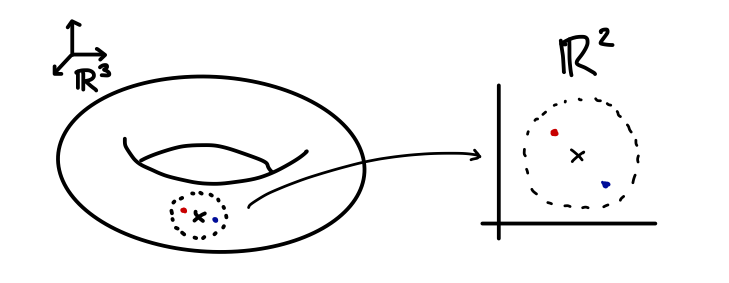
\includegraphics[width=\textwidth] {figs/charted_doughnut.png}}
    \caption{
        \label{fig:doughnut}
        Example of mapping from doughnut to $\mathbb{R}^2$ 
    }
\end{figure}

Above, I said we can "induce" a topology. This is a fanciful way of saying that
a subset takes on the topology of its parent while preserving the topological
properties, e.g. define a topology for a sphere from the Euclidean
topology of $\mathbb{R}^3$, while preserving the topological properties. 

\begin{defn}[Induced Topology]
    Let $(S, \tau_S)$ be a topological space, and $T \subseteq S$. Then, we
    define:
    $$\tau_T = \{U \cap T \mid U \in \tau_S \}$$
    It follows that $(T, \tau_T)$ is a topological space. We call it the induced
    topology of T in S.
\end{defn}

I will not rigorously prove that this definition works, however, it should be
straightforward to see that both $\emptyset$ and $T \in \tau_T$, along with
$\tau_T$ being closed under union and finite intersection.

\end{document}
